\mainchapterstyle % this line controls style of first page of chapter and including spaces and hidden page number setting (required for every chapter)
\chapter{مقدمه} % name of chapter goes here 
\pagestyle{mainheader} % rest of pages will use mainheader style which controls style settings of rest of chapter (required for every chapter )

% Chapter content including sections and subsections goes here

\section{مقدمه}
هدف از فصل مقدمه\LTRfootnote{Introduction} شرح مختصر مسئله تحقیق، اهمیت و انگیزه محقق از پرداختن به آن موضوع به
همراه اشارهای کوتاه به روش و مراحل تحقیق است. مقدمه، اولین فصل از ساختار اصلی پایان نامه‌ها / رساله
بوده و زمینه اطلاعاتی لازم برای خواننده فراهم می‌آید. در طول مقدمه باید سعی شود موضوع تحقیق با
زبانی روشن، ساده و بطور عمیق و هدفمند به خواننده معرفی شود. این فصل باید خواننده را مجذوب و
اهمیت موضوع تحقیق را آشکار سازد. در مقدمه باید با ارائه سوابق، شواهد تحقیقی و اطلاعات موجود (با ذکر)
منبع به روش منظم، منطقی و هدفدار، خواننده را جهت داد و به سوی راه حل مورد نظر هدایت کرد.
مقدمه مناسب‌ترین جا برای ارائه اختصارات و بعضی توضیحات کلی است، توضیحاتی که شاید نتوان در
مباحث دیگر در مورد آنها توضیح داد.

مقدمه، یکی از ارکان اساسی و اصلی پایان نامه است، مهم‌ترین قسمت‌های آن عبارتند از :

\subsection{عنوان تحقيق}
باید شناختی دقیق و روشن از حوزه‌ی موضوع تحقیق را عرضه دارد و خالی از هرگونه ابهام و پیچیدگی
باشد.

\subsection{مسئله تحقیق}  
وظیفه اصلی مقدمه بیان این مطلب به خواننده است که چرا انجام تحقیق را به عهده گرفته‌اید. اگر دلیل
شما برای انجام این کار پاسخگویی به سؤال مورد علاقه‌تان است، با مشکل زیادی روبه‌رو نخواهید بود. یکی از
بهترین روشها برای نوشتن مقدمۀ یک پایان‌نامه، طرح پرسش یا پرسش‌هایی مهم و اساسی است که کار
تحقیقاتی شما از آغاز تا پایان قصد پاسخ دادن به آن را دارد. گاهی می‌توانید ابتدا اهمیت موضوع را بیان و
سپس پرسش خود را در آن موضوع مطرح کنید.

\subsection{تاریخچه‌ای از موضوع تحقيق}
به طور کلی تشریح روند‌های تحقیقاتی در محدوده مورد مطالعه، مستلزم ارجاع به کارهای دیگران
است. بعضی از نویسندگان برای کارهای دیگران هیچ اعتباری قائل نمی‌شوند و در مقابل، بعضی دیگر از
نویسندگان در توصیف کارهای دیگران، بسیار زیاده‌روی می‌کنند. اکثر مواقع ارجاع به مقالات دو سال قبل از
کارتان، بهتر از نوشتن سطرها مرجع است. در این قسمت مختصری از نظرات و تحقیقات مربوط به موضوع و
یا مسائل و مشکلات حل نشده در این حوزه و همچنین توجه و علاقه جامعه به این موضوع اشاره می‌شود.

\subsection{تعريف موضوع تحقیق}
در این قسمت محقق موضوع مورد علاقه و یا نیاز احساس شده خود را در حوزه تحقیق بیان می‌دارد و
عوامل موجود در موقعیت را تعریف و تعیین می‌کند

\subsection{هدف يا هدف‌های كلی و آرمانی تحقیق}  
این قسمت باید با جملات مثبت و کلی طرح شود و از طولانی شدن مطالب پرهیز شود

\subsection{روش انجام تحقیق}
در این قسمت پژوهشگر روش کاری خود را بیان می‌دارد و شیوه‌های گوناگونی را که در گردآوری
مطالب خود به کار برده ذکر می‌کند و همچنین اگر روش آماری خاصی را در تهیه و تدوین اطلاعات به کار
برده آن شیوه را بیان می‌کند.

\subsection{نوآوری، اهمیت و ارزش تحقیق}
در این قسمت نوآوری علمی و عملی تحقیق که محقق به آن دست خواهد یافت، بحث می‌شود.
ممکن است لازم باشد تا از برخی نمودارها در این بخش استفاده شود. توجه شود، استفاده از نمودار در این
بخش تنها و تنها به جهت ارائه مثالی برای استفاده از نمودارها می‌باشد. طبیعتا به صلاحدید
نگارنده شکلها و نمودارها می‌توانند در بخش‌های مختلف مورد استفاده قرار گیرند.


% example of using charts you can change it's setting based on your porpose
\begin{chart}[H]
\centering
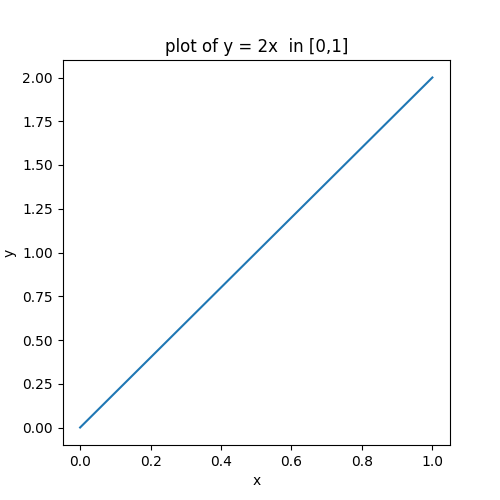
\includegraphics[width=0.7\textwidth]{images/chart_test}
\caption{نمونه‌ی استفاده از نمودار}
\label{chart:example}
\end{chart}

نمودار \ref{chart:example} نمونه‌ی استفاده از نمودار است.


\section{تعريف واژه‌ها (اختیاری)}
در این قسمت محقق باید واژه‌هایی که ممکن است برای خواننده آشنا نباشد تعریف کند


\section{خلاصه فصل‌ها}
در این قسمت خلاصه‌ای اشاره‌وار از فصل‌های آتی آورده می‌شود تا خواننده بتواند تصویری واضح از
دیگر قسمت‌های پایان‌نامه در ذهن خود ترسیم کند.
